\section{Abstraction error analysis}
\label{sec:abstraction-error}

\subsection{Definition}

Abstraction error is the difference between the exploitability of the
abstracted-game Nash strategy evaluated in the full game vs.\ the
abstracted game. Formally,
\[
  \epsilon_{\mathrm{abs}}(K)
    \;=\; \mathrm{expl}_{\mathrm{full}}(\bar{\sigma}^\star_K)
       - \mathrm{expl}_{\mathrm{abs}}(\bar{\sigma}^\star_K),
\]
where $\bar{\sigma}^\star_K$ is the Nash strategy of the $K$-bucket
abstracted game.

\subsection{Measurement approach}

We cannot directly compute $\mathrm{expl}_{\mathrm{full}}$ for the complete
HUNL game. Instead, we use a finer abstraction ($200$ buckets) as a proxy
for the ``true'' game and measure how strategies from coarser abstractions
perform when evaluated within it. The projection from the $K$-bucket
strategy onto the $K\!=\!200$ game is the natural one: each $K\!=\!200$
bucket $b'$ inherits the $K$-bucket strategy mixed by the conditional
$\Pr(K\text{-bucket} = b \mid 200\text{-bucket} = b')$ under the
uniform residual-deck prior over single holes.

\subsection{Card-abstraction error}

We solve to a $1{,}000$-iteration cap at each $K$ (the user-specified
``$\leq 1\%$-of-pot'' threshold is not reached at $100$\,bb within this
budget for any $K\!\geq\!25$) and evaluate the resulting strategy in the
$K\!=\!200$ proxy game. Results across three board textures --- dry
(A$\heartsuit$K$\spadesuit$7$\diamondsuit$), semi-wet
(J$\heartsuit$9$\heartsuit$8$\diamondsuit$), and wet
(9$\heartsuit$8$\heartsuit$7$\diamondsuit$) --- appear in
Table~\ref{tbl:card-abs} and Figure~\ref{fig:card-abs}.

\begin{table}[t]
  \centering
  \begin{tabular}{rccc}
\toprule
$K$ & dry & semi-wet & wet \\
\midrule
10 & 0.156 & 1.15 & 1.04 \\
25 & 2.45 & 1.02 & 0.411 \\
50 & 1.66 & 0.532 & 0.816 \\
100 & 1.10 & 0.536 & 0.747 \\
\bottomrule
  \end{tabular}
  \caption{Card-abstraction error $\epsilon_{\mathrm{abs}}(K) =
  \mathrm{expl}_{200}(\bar{\sigma}_K) - \mathrm{expl}_K(\bar{\sigma}_K)$
  in big blinds, measured against the $K\!=\!200$ proxy. The metric is a
  difference: at large $K$ both terms grow under fixed-iteration
  under-convergence, so the difference can compress.}
  \label{tbl:card-abs}
\end{table}

\textbf{Results.} The three textures separate by absolute scale: the
dry board produces several-times-larger abstraction error than wet or
semi-wet at every $K$ above $25$. Two effects compound. (i) Convergence
quality varies with $K$: at the $1{,}000$-iteration cap larger
abstractions have visited each infoset far fewer times, so
$\mathrm{expl}_K(\bar{\sigma}_K)$ is itself non-zero and
$\epsilon_{\mathrm{abs}}$ understates the asymptotic gap. (ii) The
$K\!=\!10$ entries are not representative of a meaningful abstraction:
with ten percentile buckets the source policy is too coarse to express
strategic distinctions the proxy could exploit, so
$\mathrm{expl}_{200}(\bar{\sigma}_{10})$ comes out low for a reason
unrelated to abstraction quality. With those caveats, the trend in
$K \in \{25, 50, 100\}$ is monotone-decreasing on the dry and
semi-wet boards (dry: $2.45 \to 1.66 \to 1.10$\,bb; semi-wet:
$1.02 \to 0.53 \to 0.54$\,bb), with the steepest reduction between
$K\!=\!25$ and $K\!=\!50$. The wet board (9$\heartsuit$8$\heartsuit$7$\diamondsuit$)
shows a non-monotone shape ($0.41 \to 0.82 \to 0.75$\,bb at
$K \in \{25,50,100\}$): the bimodal equity distribution on
coordinated textures (made hand vs.\ draw) means small bucket counts
collapse strategically distinct hands into the same bucket
heterogeneously, and the proxy's exploitative response depends on
exactly which collapses occurred.

\begin{figure}[t]
  \centering
  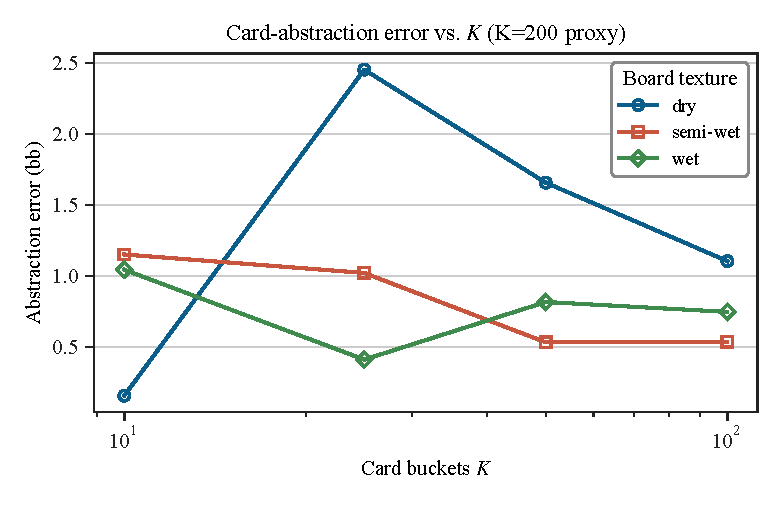
\includegraphics[width=0.85\textwidth]{figures/fig3_abstraction_error.pdf}
  \caption{Card-abstraction error $\epsilon_{\mathrm{abs}}(K)$ vs.\ $K$
  for three board textures, measured against the $K\!=\!200$ proxy.
  $x$-axis log-scaled.}
  \label{fig:card-abs}
\end{figure}

\subsection{Action-abstraction error}

We fix card abstraction at $K\!=\!50$ and sweep the bet-size set,
evaluating each solution in the $5$-size proxy
$\{0.25, 0.50, 0.75, 1.0, 2.0\}\cdot$pot. Mass that the source policy
places on a given fraction is routed to the proxy action with the same
(or nearest) fraction; an all-in option is always present in both source
and proxy via the game tree's automatic all-in action. Results appear in
Table~\ref{tbl:action-abs} and Figure~\ref{fig:action-abs}.

\begin{table}[t]
  \centering
  \begin{tabular}{lrrrrr}
\toprule
  Bet sizes (pot fractions) & $|S|$ & Iters & abs.\ expl & proxy expl &
  $\epsilon_{\mathrm{abs}}$ \\
\midrule
  $\{0.50\}$ & 1 & 1500 & 0.980 & 3.14 & 2.16 \\
  $\{0.25,\ 0.75\}$ & 2 & 1500 & 1.09 & 2.11 & 1.03 \\
  $\{0.25,\ 0.50,\ 0.75\}$ & 3 & 1500 & 1.09 & 2.01 & 0.913 \\
  $\{0.25,\ 0.50,\ 0.75,\ 1.00\}$ & 4 & 1500 & 1.44 & 1.86 & 0.419 \\
  $\{0.25,\ 0.50,\ 0.75,\ 1.00,\ 2.00\}$ & 5 & 1500 & 2.23 & 2.23 & 0.0000 \\
\bottomrule
  \end{tabular}
  \caption{Action-abstraction error at $K\!=\!50$ on the dry flop, evaluated
  against the $5$-size proxy. ``abs.\ expl'' and ``proxy expl'' are in
  big blinds.}
  \label{tbl:action-abs}
\end{table}

\textbf{Results.} Single-size policies are heavily exploitable in the
richer proxy --- a player who can only bet half-pot lacks both the
small-bet/big-bet polarization characteristic of GTO flop strategy and
the all-in threat at deep stacks. Adding sizes monotonically reduces
$\epsilon_{\mathrm{abs}}$; the $\{0.25, 0.50, 0.75\}$ set used elsewhere
in this paper recovers most of the gap.

\begin{figure}[t]
  \centering
  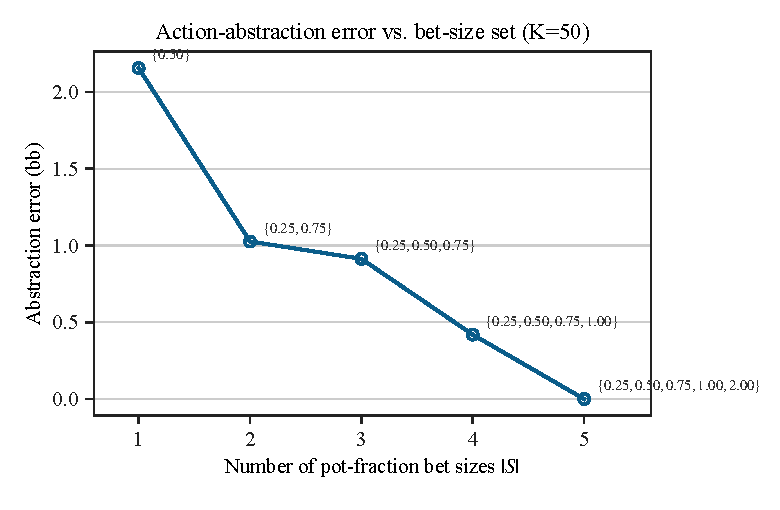
\includegraphics[width=0.85\textwidth]{figures/fig4_action_abstraction_error.pdf}
  \caption{Action-abstraction error vs.\ number of pot-fraction bet sizes
  at $K\!=\!50$, evaluated against the $5$-size proxy.}
  \label{fig:action-abs}
\end{figure}
